\chapter{DISEÑO CONCEPTUAL}\label{cap:diseno-conceptual}
\listasdecapitulo{3}

En este capítulo se establece la base conceptual de un sistema de control adaptativo inteligente para la red
semafórica vial de Lima. Siguiendo la metodología de diseño VDI 2221, se parte del análisis de los actores y
sus necesidades, se deriva una lista de requerimientos verificable, se modela el sistema como una caja negra,
se descompone su estructura funcional, y mediante una matriz morfológica se generan y evalúan conceptos
completos hasta seleccionar la solución óptima. El propósito es responder a la problemática del sistema
semafórico actual, caracterizado por ineficiencia, descoordinación y falta de adaptabilidad al flujo
vehicular.

\textbf{Qué queda fijo y qué se valida.} El diseño conceptual fija las decisiones de arquitectura del sistema
y no se modifican en los capítulos posteriores: (i) una arquitectura complementaria \emph{edge}--nube en la
que el módulo IoT recomienda y el controlador semafórico existente conserva la \textbf{autoridad final} sobre
luces y enclavamientos; (ii) el sensado principal basado en \textbf{una única cámara} con visión por
computadora; (iii) la estimación local de un índice de congestión y un \textbf{control difuso} como estrategia
de adaptación; (iv) la comunicación segura con la nube para supervisión, histórico y coordinación no crítica;
y (v) la validación mediante \textbf{SUMO} frente a una línea base. En cambio, los \emph{valores de
ingeniería} (protecciones y autonomía energética, grado IP y geometría del gabinete, altura y cobertura de la
cámara, parámetros del controlador difuso, métricas de desempeño y costos) se calculan, dimensionan y
\textbf{validan} en los Capítulos~4 a~7. Esta separación evita afirmar resultados antes de obtenerlos y
mantiene el diseño conceptual como marco estable de las etapas siguientes.

\section{Actores clave y necesidades}\label{sec:actores-necesidades}

Los actores clave del sistema se identificaron a partir de entrevistas con expertos y encuestas a usuarios del
sistema actual. Comprenden al cliente principal (la Municipalidad Metropolitana de Lima), los usuarios finales
directos (conductores y peatones), los usuarios indirectos (operativos de tránsito y administradores de la
infraestructura) y los interesados secundarios (autoridades de seguridad vial). La Tabla~\ref{tab:actores}
sintetiza sus necesidades.

\begin{table}[H]
  \centering
  \caption{Actores clave del sistema y sus necesidades principales.}
  \label{tab:actores}
  \begin{tabularx}{\linewidth}{@{}>{\raggedright\arraybackslash}p{4.3cm}>{\raggedright\arraybackslash}X@{}}
    \toprule
    \textbf{Actor} & \textbf{Necesidades principales}\\
    \midrule
    Cliente (Municipalidad / Subgerencia de Movilidad Urbana) &
    Coordinación y eficiencia de la red en tiempo real mediante ajuste dinámico de ciclos según el flujo;
    monitoreo en tiempo real interpretable, con alertas sobre incidencias y desviaciones del tráfico.\\
    Usuarios finales (conductores y peatones) &
    Reducir tiempos de espera y mejorar la fluidez, en especial en intersecciones con semáforos mal
    coordinados; mejorar la seguridad vial reduciendo accidentes y conductas temerarias asociadas a la
    frustración.\\
    Usuarios indirectos (operativos y administradores de infraestructura) &
    Comunicación centralizada para supervisar y sincronizar intersecciones desde un punto único; medidas de
    ciberseguridad que protejan la integridad y confidencialidad de los datos.\\
    Usuarios directos y operativos (autoridades de tránsito) &
    Interfaz gráfica intuitiva con alertas automáticas y datos en tiempo real que permitan un ajuste ágil y
    decisiones rápidas ante situaciones imprevistas.\\
    \bottomrule
  \end{tabularx}
  \fuente{Elaboración propia.}
\end{table}

Las respuestas de la encuesta a usuarios finales respaldan estas necesidades: el 60\,\% consideró muy
importante la reducción de tiempos de espera, el 40\,\% destacó la sincronización entre semáforos como aspecto
clave y el 50\,\% asoció las conductas peligrosas a la frustración causada por el sistema semafórico actual.

\section{Lista de requerimientos}\label{sec:requerimientos}

A partir de las necesidades anteriores se derivan los requerimientos del sistema, clasificados como exigencias
(obligatorias) o deseos (mejoras adicionales). La Tabla~\ref{tab:exigencias} resume las exigencias y deseos
por dominio de diseño, conforme a la estructura VDI 2221.

\begin{table}[H]
  \centering
  \caption{Resumen de exigencias y deseos por dominio de diseño.}
  \label{tab:exigencias}
  \begin{tabularx}{\linewidth}{@{}>{\raggedright\arraybackslash}p{2.6cm}>{\raggedright\arraybackslash}p{1.9cm}>{\raggedright\arraybackslash}X@{}}
    \toprule
    \textbf{Aspecto} & \textbf{Carácter} & \textbf{Especificación}\\
    \midrule
    Función principal & Exigencia & Sistema de semaforización adaptativa que optimiza la gestión del tráfico en
    tiempo real usando sensado IoT, comunicación con la nube y algoritmos de inteligencia artificial.\\
    Energía & Exigencia & Alimentación principal desde la red eléctrica (DC de 12\,V o 24\,V) con respaldo
    capaz de operar un mínimo de 1\,h ante corte de energía.\\
    Fuerzas & Exigencia & La estructura debe soportar el peso de placa, microcontrolador, sensores, actuadores
    y de la propia carcasa.\\
    Materia & Exigencia & Módulo resistente a temperatura, humedad, polvo y radiación solar; impermeable,
    antivandálico y con aislamiento contra cortocircuitos y daños físicos.\\
    Comunicación & Exigencia & Comunicación NTCIP entre semáforos y la plataforma centralizada, con base de
    datos para registro y análisis.\\
    Control & Exigencia & Control adaptativo que ajusta los ciclos según el tráfico en tiempo real, escalable a
    futuras intersecciones e integrando aprendizaje para mejorar la predicción de flujo.\\
    Software & Exigencia & Gestión de algoritmos de control adaptativo, procesamiento de sensores en tiempo
    real, actualización remota por la nube y ciberseguridad según estándares internacionales.\\
    Uso & Exigencia & Interoperabilidad con los semáforos y controladores existentes en Lima.\\
    Seguridad & Exigencia & Ciberseguridad según IEC 62443 y protección física del módulo frente a clima
    extremo y vandalismo (IP65).\\
    Geometría & Deseo & Módulo IoT de tamaño máximo aproximado de 70$\times$70$\times$80\,cm.\\
    Precio & Deseo & Solución de bajo costo, con presupuesto máximo estimado de 10\,000 soles por intersección.\\
    \bottomrule
  \end{tabularx}
  \fuente{Elaboración propia.}
\end{table}

Para conducir el diseño y cerrar la validación, las exigencias anteriores se traducen en una
\textbf{especificación verificable codificada} (Tabla~\ref{tab:req-verificables}), donde cada requerimiento
recibe un código, un valor objetivo o criterio, su justificación y el método de verificación previsto. La
prioridad se clasifica como M (mandatoria), A (alta) o D (deseable). Esta tabla presenta la versión
consolidada que gobierna el resto de la tesis; el desglose fino por subcriterio y las hojas de cálculo
asociadas se incluyen en el Anexo de requerimientos.

\begin{landscape}
\footnotesize
\begin{longtable}{@{}p{1.15cm}p{1.7cm}p{5.1cm}p{3.1cm}p{4.2cm}p{3.6cm}p{1.0cm}@{}}
\caption{Requerimientos verificables del módulo IoT semafórico.}\label{tab:req-verificables}\\
\toprule
\textbf{Código} & \textbf{Categoría} & \textbf{Requerimiento} & \textbf{Valor objetivo o criterio} & \textbf{Justificación} & \textbf{Método de verificación} & \textbf{Prior.}\\
\midrule
\endfirsthead
\toprule
\textbf{Código} & \textbf{Categoría} & \textbf{Requerimiento} & \textbf{Valor objetivo o criterio} & \textbf{Justificación} & \textbf{Método de verificación} & \textbf{Prior.}\\
\midrule
\endhead
\bottomrule
\endfoot
R-F01 & Funcional & Estimar el estado de congestión local a partir de video o variables equivalentes de tráfico. & Flujo, velocidad, ocupación y/o cola por acceso. & El control adaptativo requiere una medida local de demanda y acumulación. & Escenarios SUMO y prueba del algoritmo de visión con datos etiquetados. & M\\
R-F02 & Funcional & Calcular un índice de congestión local como entrada del controlador. & Índice normalizado y documentado; pesos calibrados o justificados. & Permite combinar variables heterogéneas en una entrada interpretable. & Revisión de ecuaciones, análisis de sensibilidad y casos de prueba. & M\\
R-F03 & Funcional & Generar telemetría, estado del módulo, alertas y registros históricos. & Estructura de mensajes definida y con marca temporal. & La supervisión y el mantenimiento requieren trazabilidad operacional. & Inspección de mensajes, base de datos y dashboard controlado. & A\\
R-C01 & Control & Generar localmente tiempos o parámetros de fase recomendados sin depender de la nube. & Decisión local disponible durante desconexión simulada. & Evita que la conectividad externa sea un punto único de falla. & Prueba de pérdida de enlace y revisión del flujo de control. & M\\
R-C02 & Seguridad funcional & Mantener al controlador semafórico existente como autoridad final sobre luces, enclavamientos, fases incompatibles y modos seguros. & Sin conexión directa del módulo IoT a lámparas en la arquitectura operacional. & Separa la optimización de la función certificada de seguridad vial. & Diagrama de arquitectura, interfaces y análisis de modos de falla. & M\\
R-C03 & Control & Respetar límites mínimos, máximos y tiempos de despeje para cada fase. & Valores mínimos, máximos y de despeje definidos y validados en el Capítulo~6 según norma y controlador objetivo. & Impide recomendaciones fuera del dominio operacional permitido. & Revisión de reglas, saturaciones y barrido de entradas. & M\\
R-C04 & Control & Retornar al plan base cuando la calidad de sensado sea insuficiente o exista una falla no recuperable del módulo. & Transición determinista a modo degradado. & Una estimación inválida no debe provocar ajustes no confiables. & Inyección simulada de datos ausentes o fuera de rango. & M\\
R-COM01 & Comunicación & Transmitir telemetría, métricas de tráfico, alertas y estado del equipo hacia la plataforma de supervisión. & MQTT/TLS o protocolo equivalente; frecuencia de publicación configurable. & La nube cumple funciones de supervisión e histórico, no de seguridad funcional. & Revisión de tópicos, carga útil y prueba de intercambio. & A\\
R-COM02 & Comunicación & Recibir únicamente parámetros autorizados, versionados y validados. & Lista blanca, rango permitido, vigencia y firma/token verificable. & Reduce el riesgo de manipulación remota de la configuración. & Casos de aceptación/rechazo de parámetros. & M\\
R-NUB01 & Nube & Almacenar históricos, mostrar estado, gestionar alertas y apoyar coordinación no crítica. & Disponibilidad acorde a un servicio de supervisión no crítico, sin cerrar el lazo de seguridad. & Centraliza análisis y operación sin cerrar el lazo crítico en la nube. & Demostración en entorno controlado y revisión de arquitectura. & A\\
R-SEC01 & Ciberseguridad & Proteger comunicaciones mediante cifrado, autenticación mutua o equivalente y control de acceso. & TLS vigente, credenciales por dispositivo y roles de usuario. & Protege confidencialidad, integridad y autenticidad. & Revisión de configuración, flujo de autenticación y modelo de amenazas. & M\\
R-SEC02 & Ciberseguridad & Contemplar pérdida de conectividad, datos falsos, acceso no autorizado y manipulación de parámetros. & Amenazas registradas con mitigación y verificación. & Son escenarios plausibles en infraestructura IoT urbana. & Tabla de amenazas y pruebas negativas controladas. & M\\
R-SEC03 & Ciberseguridad & Registrar accesos, cambios de configuración, errores y eventos relevantes. & Logs con identidad, fecha, acción y resultado. & Permite auditoría y análisis posterior de incidentes. & Inspección de registros y trazabilidad de una operación. & A\\
R-SEC04 & Ciberseguridad & Aplicar mínimo privilegio y separación entre recomendación y actuación. & Roles diferenciados; ningún usuario del dashboard gobierna directamente las lámparas. & Limita el impacto de una cuenta comprometida. & Revisión de permisos y diagrama de confianza. & M\\
R-ELEC01 & Electrónico & Incorporar protecciones contra sobrecorriente, sobretensión y fallas de alimentación. & Protecciones dimensionadas por cálculo en el Capítulo~4. & El entorno vial presenta transitorios y operación continua. & Esquema eléctrico, hojas de datos y coordinación de protecciones. & M\\
R-ELEC02 & Electrónico & Disponer de respaldo energético para apagado controlado o continuidad temporal del módulo. & Autonomía dimensionada según perfil de carga en el Capítulo~4. & Evita pérdida abrupta de registros y diagnósticos. & Balance de potencia y cálculo de batería/UPS. & A\\
R-ELEC03 & Electrónico & Separar alimentación de potencia, señales y comunicaciones, incorporando diagnóstico interno. & Canalización y puntos de medición documentados. & Reduce interferencia y facilita mantenimiento. & Revisión de PCB, esquema y distribución interna. & A\\
R-MEC01 & Mecánico & Alojar los componentes con acceso de mantenimiento, ventilación y reserva de expansión. & Gabinete modular; volumen y holguras definidos en CAD en el Capítulo~5. & La mantenibilidad condiciona el costo de operación. & CAD, plano de distribución y procedimiento de acceso. & A\\
R-MEC02 & Mecánico & Proteger los componentes frente a polvo, humedad, radiación y manipulación. & Grado IP65 objetivo y resistencia al impacto, validados en el Capítulo~5. & La instalación prevista es exterior y accesible. & Especificación de gabinete, sellos, material y análisis de riesgos. & M\\
R-MEC03 & Mecánico & Posicionar la cámara con cobertura de las zonas de interés sin comprometer estabilidad. & Campo visual y cobertura validados con geometría y prueba en el Capítulo~5. & La calidad de estimación depende del encuadre y la oclusión. & CAD, cobertura, análisis estructural y prueba de campo. & A\\
R-OP01 & Operación & Permitir mantenimiento, actualización y recuperación sin alterar la programación segura del controlador vial. & Procedimiento documentado y configuración respaldada. & Reduce tiempo fuera de servicio y riesgo operacional. & Revisión de procedimiento y prueba en banco. & A\\
R-VAL01 & Validación & Comparar el control propuesto con una estrategia fija o convencional bajo la misma demanda. & Casos A y B con semilla y horizonte comunes. & La mejora solo es defendible frente a una línea base reproducible. & Simulación SUMO/TraCI y archivos de configuración. & M\\
R-VAL02 & Validación & Reportar espera, colas, velocidad, throughput, paradas, viaje, ICV y consumo/emisiones cuando estén disponibles. & Tabla comparativa con unidades y dispersión. & Evita sustentar el desempeño en una única métrica. & Exportación SUMO y procesamiento estadístico. & M\\
R-VAL03 & Validación & Evaluar un caso de pérdida de conectividad y retorno al modo local/base. & Sin estados incompatibles ni dependencia de respuesta cloud. & Verifica la premisa de disponibilidad de la arquitectura edge. & Caso D simulado y registro de transición. & M\\
R-COST01 & Costos & Estimar CAPEX y OPEX por intersección, separando módulo, instalación, conectividad, nube y mantenimiento. & Valores con fuente, fecha y supuestos, detallados en el Capítulo~7. & Permite evaluar viabilidad y escalamiento. & Hoja de costos y análisis de sensibilidad. & A\\
\end{longtable}
\fuente{Elaboración propia.}
\end{landscape}

\section{Estructura de funciones}\label{sec:estructura-funciones}

\subsection{Frontera del sistema y modelo de caja negra}\label{sec:caja-negra}

La frontera del sistema se fija alrededor del módulo IoT complementario. El controlador semafórico existente y
la plataforma en la nube son sistemas externos con los que se intercambian señales; las lámparas y sus
enclavamientos permanecen bajo responsabilidad del controlador vial. La Figura~\ref{fig:caja-negra} representa
el sistema como una caja negra, en la que las líneas punteadas representan señales, las líneas delgadas la
energía y las líneas gruesas la materia.

\begin{figure}[H]
  \centering
  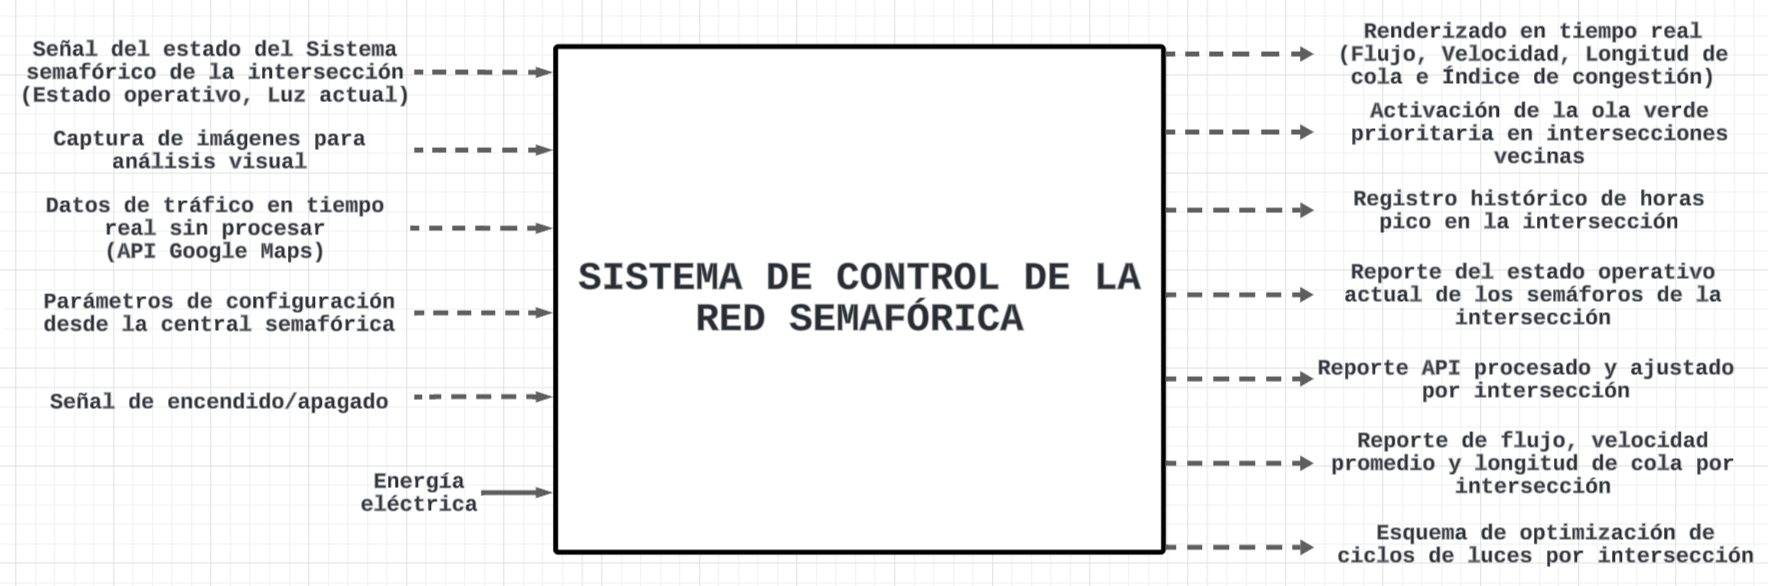
\includegraphics[width=0.9\linewidth,keepaspectratio]{media/image91.png}
  \caption{Caja negra del sistema y frontera de responsabilidad del módulo IoT complementario.}
  \label{fig:caja-negra}
  \fuente{Elaboración propia.}
\end{figure}

La Tabla~\ref{tab:entradas-salidas} consolida las entradas y salidas del sistema con su uso dentro de la
arquitectura, evitando duplicar en prosa el detalle de cada señal.

\begin{table}[H]
  \centering
  \caption{Entradas y salidas del módulo IoT y su uso dentro de la arquitectura.}
  \label{tab:entradas-salidas}
  \begin{tabularx}{\linewidth}{@{}>{\raggedright\arraybackslash}p{1.7cm}>{\raggedright\arraybackslash}p{5.0cm}>{\raggedright\arraybackslash}X@{}}
    \toprule
    \textbf{Tipo} & \textbf{Variable o flujo} & \textbf{Uso dentro de la arquitectura}\\
    \midrule
    Entrada & Imagen o video de la cámara & Estimar conteo, velocidad, ocupación, cola y calidad del sensado.\\
    Entrada & Sensores auxiliares y diagnóstico eléctrico/ambiental & Detectar condiciones internas anómalas y apoyar el mantenimiento.\\
    Entrada & Estado del controlador semafórico & Sincronizar recomendaciones con la fase vigente sin sustituir sus enclavamientos.\\
    Entrada & Parámetros autorizados e históricos & Configurar límites, pesos y referencias dentro de rangos validados.\\
    Entrada & Restricciones de seguridad y estado de conectividad & Seleccionar modo normal, degradado o retorno al plan base.\\
    Entrada & Energía eléctrica & Alimentar de forma estable y continua a todos los componentes.\\
    Salida & Índice de congestión y variables de tráfico & Entradas verificables para el control difuso y la supervisión.\\
    Salida & Parámetros sugeridos de fase & Recomendación acotada que debe ser validada por la autoridad final.\\
    Salida & Telemetría, alertas, reportes y estado del módulo & Operación, mantenimiento, auditoría y análisis histórico.\\
    Salida & Registro local e histórico remoto & Evidencia para trazabilidad, diagnóstico y calibración.\\
    \bottomrule
  \end{tabularx}
  \fuente{Elaboración propia.}
\end{table}

\subsection{Descomposición funcional por dominios}\label{sec:dominios-funcionales}

La estructura funcional se organiza en dominios complementarios: \textbf{sensado}, que capta la escena vial;
\textbf{procesamiento local}, que preprocesa y estima variables; \textbf{control}, que calcula el ajuste
difuso y aplica restricciones; \textbf{comunicación}, que intercambia mensajes; \textbf{nube}, que supervisa y
conserva históricos; \textbf{ciberseguridad}, que protege identidad, acceso, integridad y registros;
\textbf{energía}, que alimenta, convierte, respalda y protege; \textbf{mecánico}, que soporta y protege
sensores y electrónica; y \textbf{operación y mantenimiento}, que diagnostica, actualiza y recupera el sistema.
Las funciones internas mínimas son captar la escena vial; preprocesar datos; estimar flujo, cola, velocidad u
ocupación; calcular el índice de congestión; ejecutar el control difuso local; validar restricciones de
seguridad; comunicar telemetría; recibir parámetros autorizados; registrar eventos; gestionar fallos de
comunicación y sensado; proteger accesos y datos; alimentar y proteger componentes; y soportar físicamente la
cámara y la electrónica.

La Figura~\ref{fig:estructura-funciones} muestra la estructura de funciones global, que sigue la misma
convención de líneas de la caja negra (señales punteadas, energía delgada, materia gruesa). El flujo general
se inicia con la activación y distribución de energía a interfaz, sensores, control y actuadores; a partir de
allí el sistema recibe video y señales de estado, estima las variables de tráfico, calcula el índice de
congestión, ejecuta el control difuso y, mediante la central semafórica, comunica recomendaciones acotadas al
controlador, que es quien finalmente acciona las luces.

\begin{figure}[H]
  \centering
  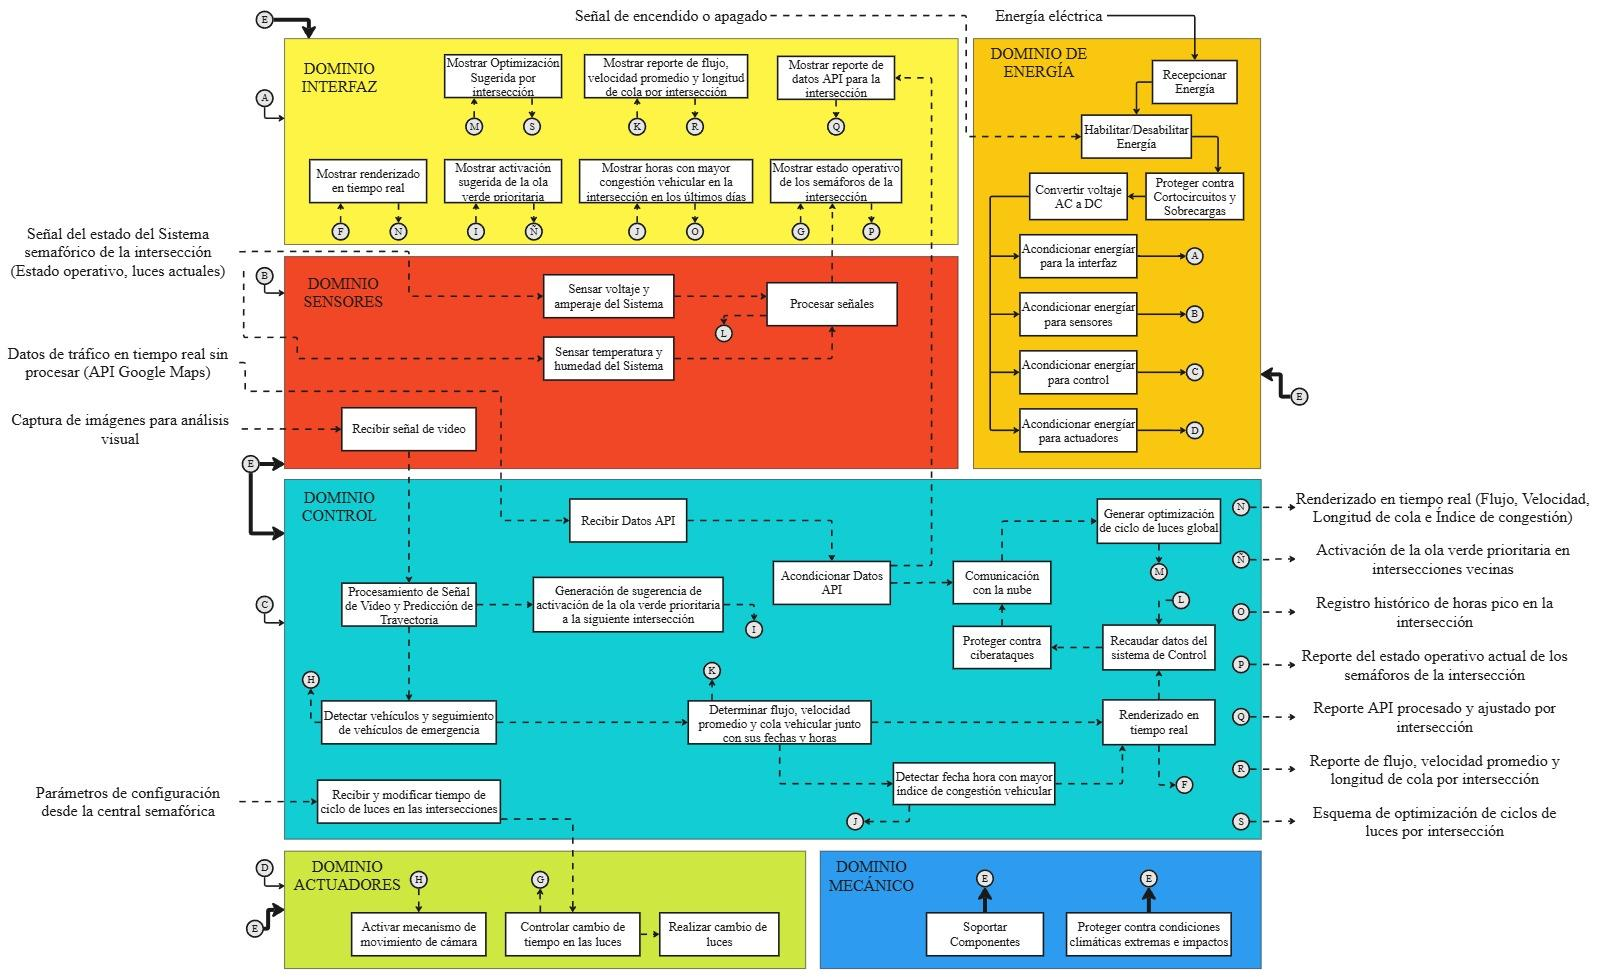
\includegraphics[width=0.9\linewidth,keepaspectratio]{media/image154.jpg}
  \caption{Estructura de funciones global del sistema, organizada por dominios.}
  \label{fig:estructura-funciones}
  \fuente{Elaboración propia.}
\end{figure}

Las señales internas que enlazan los dominios en el diagrama se identifican con letras. La
Tabla~\ref{tab:senales-funciones} reúne su significado, integrando en una sola referencia la nomenclatura que
en versiones anteriores aparecía dispersa en el texto.

\begin{table}[H]
  \centering
  \caption{Significado de las señales internas de la estructura de funciones.}
  \label{tab:senales-funciones}
  \begin{tabularx}{\linewidth}{@{}cX@{}}
    \toprule
    \textbf{Señal} & \textbf{Significado}\\
    \midrule
    A--D & Acondicionar energía para interfaz (A), sensores (B), control (C) y actuadores (D).\\
    E & Señal mecánica de soporte y protección contra condiciones extremas e impactos.\\
    F & Renderizado en tiempo real de las variables de tráfico.\\
    G & Cambio de tiempo en las luces.\\
    H & Seguimiento visual continuo del vehículo de emergencia.\\
    I & Generación de sugerencia para la activación de la ola verde prioritaria.\\
    J & Índice de congestión vehicular por fecha y hora.\\
    K & Reporte de flujo, velocidad promedio y longitud de cola por intersección.\\
    L & Datos acondicionados del estado del sistema semafórico.\\
    M & Generación de optimización del ciclo de luces global.\\
    N--S & Señales hacia la interfaz para mostrar: renderizado en tiempo real (N), activación sugerida de la ola verde (Ñ), horas de mayor congestión (O), estado operativo de los semáforos (P), reporte de datos de la API por intersección (Q), reporte de flujo, velocidad y cola (R) y optimización sugerida por intersección (S).\\
    \bottomrule
  \end{tabularx}
  \fuente{Elaboración propia.}
\end{table}

A partir de esta estructura global, cada dominio se detalla en su propio diagrama de funciones. El
\textbf{dominio de interfaz} (Figura~\ref{fig:dominio-interfaz}) agrupa las funciones de visualización para el
operador: renderizado en tiempo real, optimización sugerida por intersección, estado operativo de los
semáforos, reporte de flujo/velocidad/cola, activación sugerida de ola verde prioritaria, horas de mayor
congestión y reporte de datos de la API.

\begin{figure}[H]
  \centering
  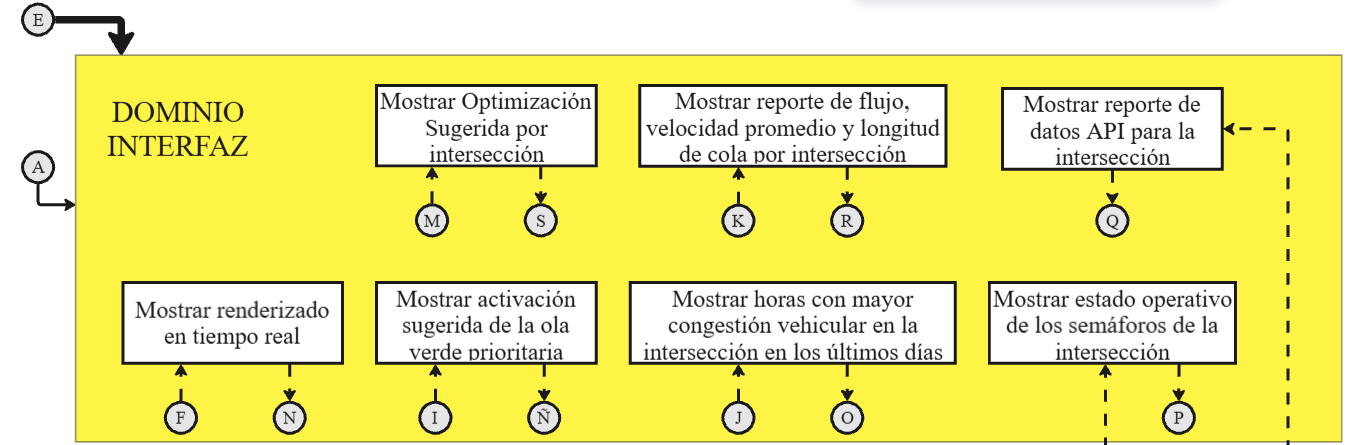
\includegraphics[width=0.9\linewidth,keepaspectratio]{media/image27.png}
  \caption{Estructura de funciones del dominio de interfaz.}
  \label{fig:dominio-interfaz}
  \fuente{Elaboración propia.}
\end{figure}

El \textbf{dominio de sensores} (Figura~\ref{fig:dominio-sensores}) recibe la señal de video, sensa voltaje y
amperaje, sensa temperatura y humedad, y procesa las señales para detectar fallas, desconexiones o anomalías
del sistema.

\begin{figure}[H]
  \centering
  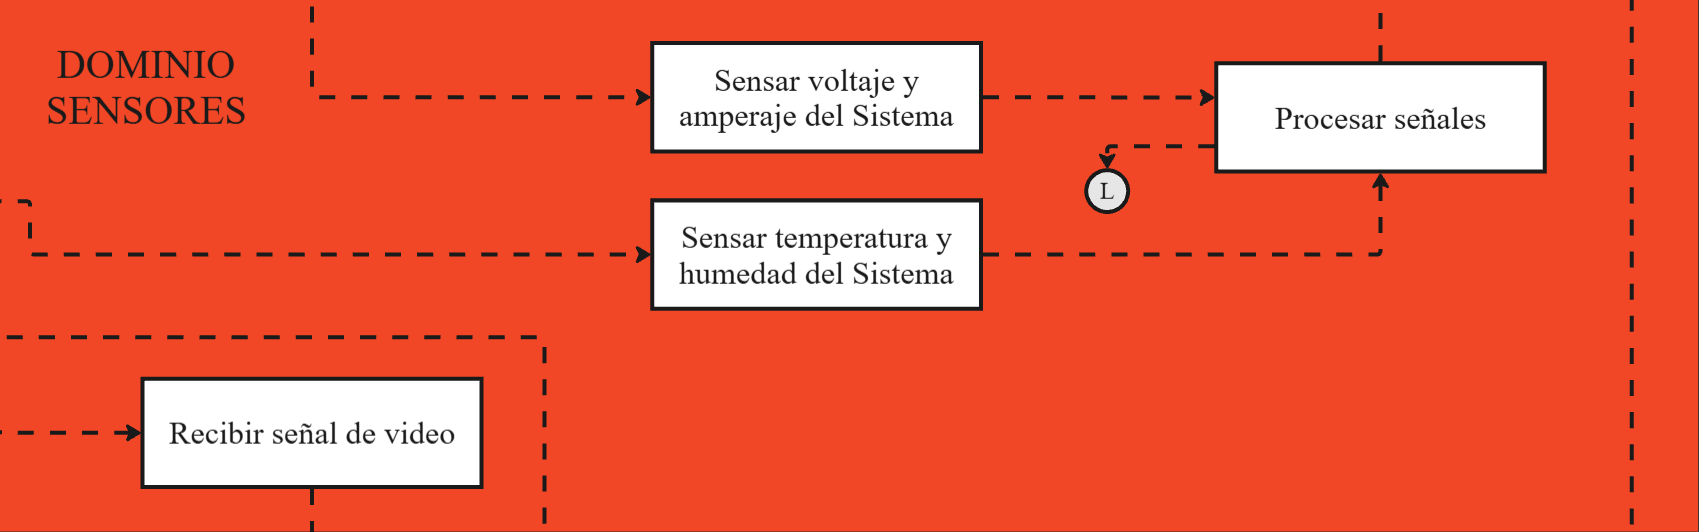
\includegraphics[width=0.9\linewidth,keepaspectratio]{media/image74.png}
  \caption{Estructura de funciones del dominio de sensores.}
  \label{fig:dominio-sensores}
  \fuente{Elaboración propia.}
\end{figure}

El \textbf{dominio de energía} (Figura~\ref{fig:dominio-energia}) recepciona la energía de la red, habilita o
deshabilita el suministro, protege contra cortocircuitos y sobrecargas, convierte AC a DC y transforma la
energía para interfaz, sensores, control y actuadores.

\begin{figure}[H]
  \centering
  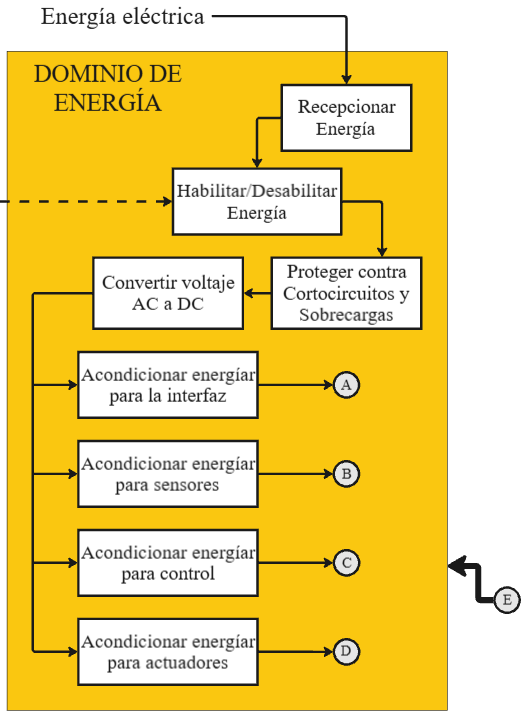
\includegraphics[width=0.9\linewidth,keepaspectratio]{media/image83.png}
  \caption{Estructura de funciones del dominio de energía.}
  \label{fig:dominio-energia}
  \fuente{Elaboración propia.}
\end{figure}

El \textbf{dominio de control} (Figura~\ref{fig:dominio-control}) constituye el núcleo: acondiciona los datos
externos, detecta y sigue vehículos, procesa el video y predice trayectorias, determina flujo, velocidad y
cola con fecha y hora, calcula el índice de congestión, genera el renderizado y las recomendaciones de
optimización, protege contra ciberataques y comunica con la nube. Sus salidas son recomendaciones acotadas,
nunca acciones directas sobre las lámparas.

\begin{figure}[H]
  \centering
  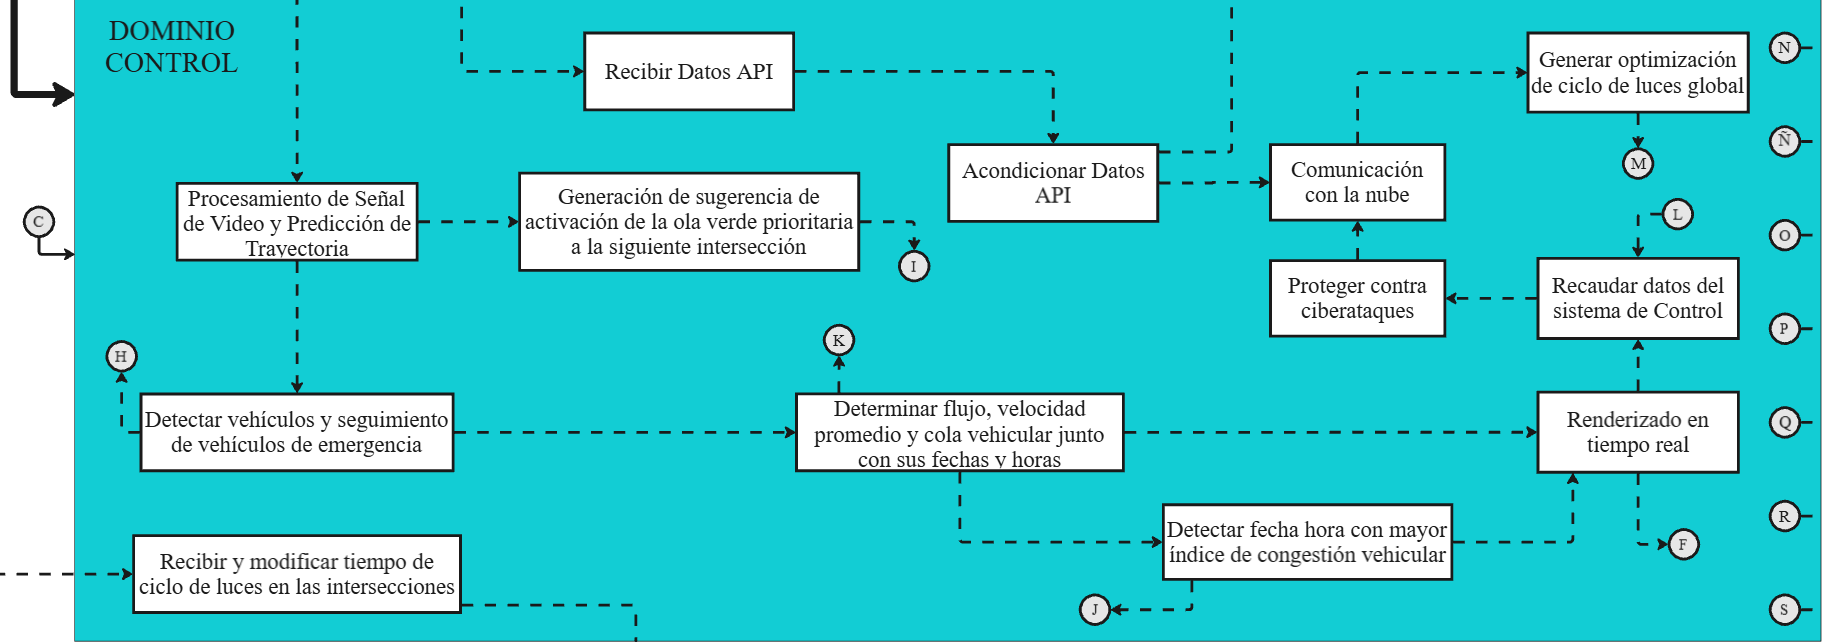
\includegraphics[width=0.9\linewidth,keepaspectratio]{media/image80.png}
  \caption{Estructura de funciones del dominio de control.}
  \label{fig:dominio-control}
  \fuente{Elaboración propia.}
\end{figure}

Finalmente, el \textbf{dominio de actuadores y el dominio mecánico} (Figura~\ref{fig:dominio-actuadores})
ejecutan, sujetos al controlador vial, el cambio de tiempos y de luces y el movimiento de la cámara, y
proveen la estructura física que soporta y protege los componentes frente a clima extremo, impactos y
vandalismo.

\begin{figure}[H]
  \centering
  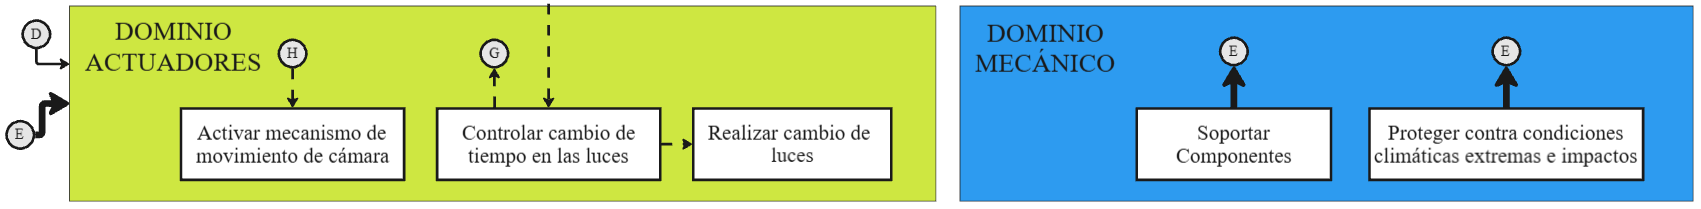
\includegraphics[width=0.9\linewidth,keepaspectratio]{media/image147.png}
  \caption{Estructura de funciones de los dominios de actuadores y mecánico.}
  \label{fig:dominio-actuadores}
  \fuente{Elaboración propia.}
\end{figure}

\section{Matriz morfológica y selección de alternativa}\label{sec:matriz-morfologica}

La matriz morfológica (Tabla~\ref{tab:matriz-morfologica}) vincula cada función principal con tecnologías
capaces de realizarla. Su propósito no es listar componentes de forma aislada, sino generar conceptos
completos y comparables. La alternativa seleccionada para el concepto óptimo se resalta en negrita.

\begin{landscape}
\footnotesize
\begin{longtable}{@{}p{3.8cm}p{3.8cm}p{3.8cm}p{3.8cm}p{3.8cm}p{3.8cm}@{}}
\caption{Matriz morfológica del sistema.}\label{tab:matriz-morfologica}\\
\toprule
\textbf{Función} & \textbf{Alternativa 1} & \textbf{Alternativa 2} & \textbf{Alternativa 3} & \textbf{Alternativa 4} & \textbf{Alternativa 5}\\
\midrule
\endfirsthead
\toprule
\textbf{Función} & \textbf{Alternativa 1} & \textbf{Alternativa 2} & \textbf{Alternativa 3} & \textbf{Alternativa 4} & \textbf{Alternativa 5}\\
\midrule
\endhead
\bottomrule
\endfoot
Sensar tráfico & \textbf{Cámara IP con visión} & Radar & Lazo inductivo & Ultrasónico/LiDAR & API externa\\
Procesar localmente & Microcontrolador & \textbf{SBC/edge computer} & Mini PC industrial & FPGA & 100\,\% nube\\
Estimar congestión & Umbrales simples & \textbf{Índice multivariable} & Modelo estadístico & Red neuronal & Dato externo\\
Adaptar tiempos & Control fijo & Actuado por demanda & \textbf{Control difuso} & Optimización matemática & Aprendizaje por refuerzo\\
Interfaz con controlador & Contactos/relés directos & Protocolo propietario & \textbf{Interfaz validada/NTCIP cuando sea compatible} & API del fabricante & Sin integración\\
Comunicar al exterior & Ethernet & Wi-Fi & \textbf{4G/LTE con respaldo o Ethernet disponible} & LoRaWAN & Fibra\\
Supervisar y almacenar & Servidor local & \textbf{Nube/híbrido} & Azure & AWS/GCP & Sin histórico\\
Proteger comunicaciones & Usuario/contraseña & TLS + token & \textbf{TLS + identidad por dispositivo + roles} & VPN + certificados & Sin seguridad explícita\\
Respaldar energía & Sin respaldo & Capacitor de retención & \textbf{UPS/batería dimensionada} & Generador & Alimentación dual\\
Proteger físicamente & Caja comercial interior & Gabinete plástico & \textbf{Gabinete metálico modular exterior} & Rack abierto & Gabinete del controlador existente\\
Validar control & Cálculo manual & \textbf{SUMO/TraCI} & VISSIM & AIMSUN & Prueba en vía pública\\
\bottomrule
\end{longtable}
\fuente{Elaboración propia.}
\end{landscape}

\subsection{Conceptos generados}\label{sec:conceptos-generados}

\begin{itemize}
  \item \textbf{Concepto A --- control centralizado en nube:} cámaras económicas transmiten datos hacia la
  nube, donde se calcula el control. Presenta alta escalabilidad informática, pero dependencia crítica de
  conectividad y mayor exposición de datos.
  \item \textbf{Concepto B --- solución industrial local cerrada:} radar o lazos, PLC/controlador industrial y
  red cableada, con mínima participación de nube. Ofrece alta robustez local, pero eleva el costo de obra e
  integración y limita la experimentación académica.
  \item \textbf{Concepto C --- módulo complementario edge--nube:} cámara, procesamiento local, índice de
  congestión, control difuso, comunicación segura con nube, gabinete modular y controlador vial como autoridad
  final.
  \item \textbf{Concepto D --- control directo basado en aprendizaje:} visión y aprendizaje por refuerzo
  generan acciones de fase. Su potencial es alto, pero exige datos, validación y garantías que exceden el
  alcance y no ofrece la interpretabilidad requerida como núcleo de esta tesis.
\end{itemize}

\subsection{Evaluación técnico-económica ponderada}\label{sec:evaluacion-ponderada}

La calificación emplea una escala de 1 a 5, donde 1 representa desempeño insuficiente y 5 desempeño muy
favorable. Los pesos expresan prioridad de diseño, no resultados experimentales. La puntuación normalizada se
calcula mediante $\sum w_i p_i/5$, con $\sum w_i = 100$.

\begin{landscape}
\footnotesize
\begin{longtable}{@{}p{5.0cm}rccccp{5.0cm}@{}}
\caption{Evaluación ponderada de conceptos de solución.}\label{tab:evaluacion-conceptos}\\
\toprule
\textbf{Criterio} & \textbf{Peso (\%)} & \textbf{A} & \textbf{B} & \textbf{C} & \textbf{D} & \textbf{Razón del peso}\\
\midrule
\endfirsthead
\toprule
\textbf{Criterio} & \textbf{Peso (\%)} & \textbf{A} & \textbf{B} & \textbf{C} & \textbf{D} & \textbf{Razón del peso}\\
\midrule
\endhead
\bottomrule
\endfoot
Adecuación a la función principal & 18 & 3 & 4 & 5 & 4 & Debe estimar tráfico y producir ajustes verificables.\\
Operación local y tiempo de respuesta & 14 & 1 & 5 & 5 & 3 & La decisión no puede depender de conectividad externa.\\
Seguridad funcional y modos degradados & 14 & 2 & 5 & 5 & 1 & El controlador existente debe conservar la autoridad final.\\
Integración con infraestructura existente & 12 & 3 & 4 & 5 & 3 & Lima presenta controladores y redes heterogéneos.\\
Mantenibilidad & 10 & 3 & 4 & 4 & 2 & El municipio requiere diagnóstico y reemplazo modular.\\
Ciberseguridad & 10 & 3 & 4 & 5 & 2 & La conectividad amplía la superficie de ataque.\\
Escalabilidad & 8 & 5 & 2 & 5 & 4 & Se busca una arquitectura replicable por intersección.\\
Costo y disponibilidad & 8 & 4 & 2 & 4 & 2 & La tesis requiere componentes disponibles y un piloto viable.\\
Facilidad de validación académica & 6 & 3 & 4 & 5 & 3 & Debe verificarse con herramientas y métricas reproducibles.\\
\midrule
\textbf{Puntuación normalizada /100} & \textbf{100} & \textbf{56.4} & \textbf{79.2} & \textbf{96.4} & \textbf{54.0} & ---\\
\bottomrule
\end{longtable}
\fuente{Elaboración propia.}
\end{landscape}

El concepto C obtiene la mayor puntuación (96,4/100) porque combina autonomía local, interpretabilidad,
compatibilidad con la validación en SUMO, supervisión remota y separación de responsabilidades. Por tanto, la
solución seleccionada es: \textbf{cámara con visión por computadora + procesamiento local en el borde + índice
de congestión + control difuso + comunicación segura con nube + SUMO como simulador + gabinete modular +
arquitectura complementaria al controlador existente}. Esta elección no implica que cada componente comercial
esté ya certificado; indica que el concepto satisface mejor los requerimientos del alcance de tesis.

\section{Solución óptima}\label{sec:solucion-optima}

La solución óptima corresponde al concepto C. Se trata de un módulo mecatrónico instalado en la intersección,
con cámara y gabinete de protección. La altura de 6,5\,m y el grado IP65 se adoptan como objetivos de diseño y
se confirman en la etapa de integración mecánica (Capítulo~5). La Figura~\ref{fig:bosquejo} muestra una
visualización del concepto.

El núcleo del sistema es un módulo IoT basado en \textbf{Raspberry Pi 5}, empleado como unidad de
procesamiento local (\emph{edge}) para adquisición de datos, visión por computadora, diagnóstico y generación
de recomendaciones de control. El módulo no reemplaza al controlador semafórico existente ni asume la
autoridad final sobre los cambios de fase: lo complementa con información procesada, parámetros sugeridos y
alertas verificables por la central semafórica. Incorpora una pantalla TFT integrada que facilita el
diagnóstico del operario en sitio, mostrando únicamente el estado operativo de los semáforos y del controlador
para mantenimiento básico. El monitoreo energético se realiza con el sensor de voltaje y corriente
\textbf{INA219}, que mide hasta $+26$\,V DC y corrientes de $\pm 3{,}2$\,A con resolución de 0,8\,mA,
alimentación de 3,0 a 5,5\,V DC, ADC interno de 12\,bits, comunicación I\textsuperscript{2}C y precisión
típica de $\pm 0{,}5\,\%$, lo que habilita un mantenimiento preventivo del consumo del módulo.

El monitoreo ambiental se realiza con el sensor de temperatura y humedad \textbf{SHT31}, que opera de 2,15 a
5,5\,V DC y ofrece precisión de $\pm 0{,}3\,^{\circ}$C y $\pm 2\,\%$ de humedad relativa (20--80\,\% RH), con
rango de $-40$ a $+125\,^{\circ}$C, comunicación I\textsuperscript{2}C y tiempo de respuesta menor a 8\,s,
adecuado para las condiciones de Lima Metropolitana.

La captura de imágenes se realiza mediante una \textbf{cámara domo IP tipo Hikvision con visión por
computadora}, apta para exteriores y con función PTZ (\emph{pan-tilt-zoom}) motorizada integrada, que cubre
las zonas de interés de la intersección y permite el seguimiento dinámico de vehículos de emergencia sin
recurrir a un soporte de servomotores externo. Esta cámara, conectada por interfaz IP/Ethernet, alimenta los
algoritmos de visión que estiman flujo vehicular, velocidad promedio y longitud de cola, y detectan vehículos
de emergencia. La altura de 6,5\,m busca maximizar la cobertura de la zona de interés; la cobertura final se
verifica mediante calibración geométrica de la cámara, pruebas de campo controladas y ajuste de las zonas de
detección, en especial en intersecciones con geometrías irregulares. Esta cámara domo IP es la
\textbf{única solución de visión} empleada de forma consistente en todo el documento.

\begin{figure}[H]
  \centering
  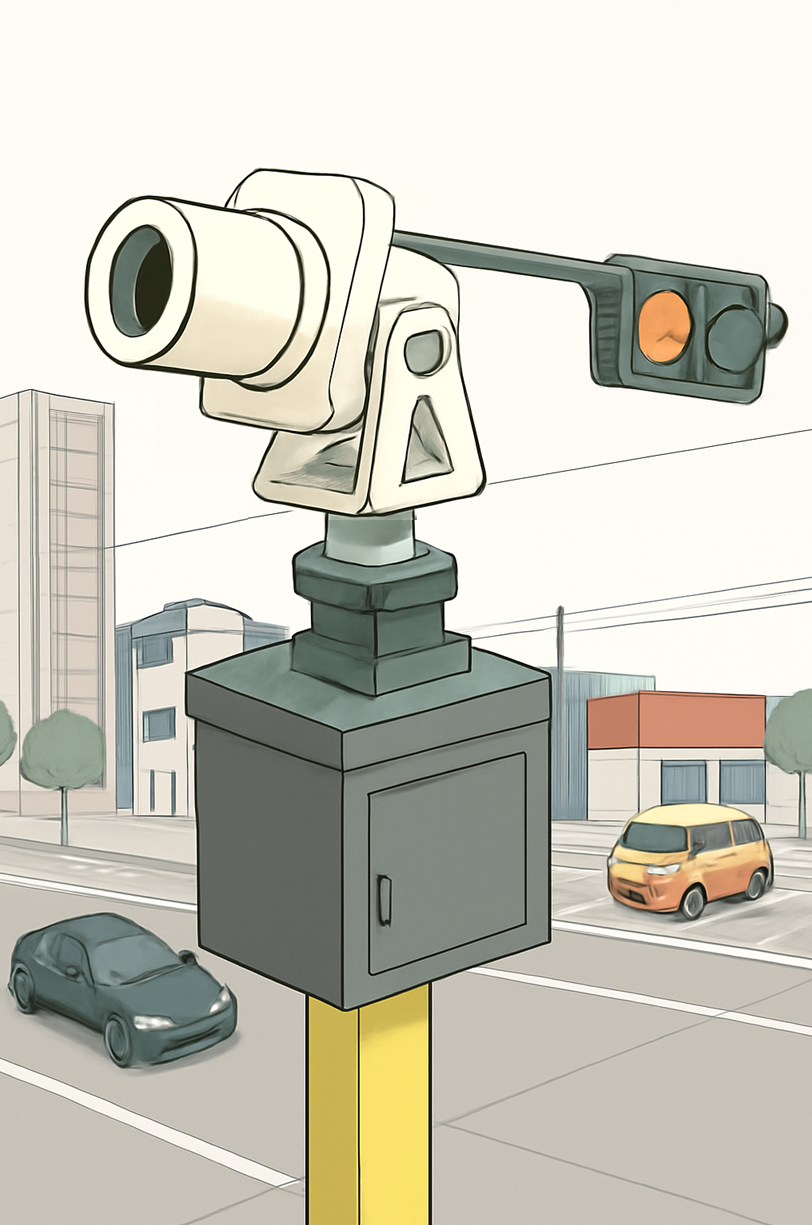
\includegraphics[width=0.9\linewidth,keepaspectratio]{media/image140.png}
  \caption{Bosquejo del diseño de la solución óptima.}
  \label{fig:bosquejo}
  \fuente{Elaboración propia.}
\end{figure}

Para el banco de pruebas y la etapa de diseño electrónico se considera una interfaz de conmutación mediante
relés de estado sólido (SSR), por su conmutación silenciosa y ausencia de desgaste mecánico. En una
implementación vial real, la actuación final de las luces permanece condicionada por el controlador
semafórico certificado, sus enclavamientos de seguridad y las restricciones normativas aplicables. La
iluminación semafórica se plantea mediante un sistema de fibra óptica LED que distribuye uniformemente la luz
desde la base del controlador hacia los focos, lo que facilita el mantenimiento.

La alimentación del sistema incorpora llaves termomagnéticas, protección diferencial o equivalente según la
instalación, una fuente AC/DC y convertidores DC/DC para los niveles requeridos. El respaldo mediante batería
o UPS se dimensiona con el perfil de carga en el Capítulo~4. La comunicación entre el controlador programable
y la central semafórica, y entre el controlador y el módulo IoT, se establece mediante el protocolo
\textbf{NTCIP} sobre TCP/IP; la comunicación entre el módulo IoT y la nube usa el protocolo \textbf{MQTT} sobre
TCP/IP con TLS, priorizando una transmisión eficiente y segura sin requerir comunicación bidireccional
constante.

El procesamiento local se plantea con OpenCV y un detector de objetos ejecutado en la unidad \emph{edge}, para
estimar flujo, velocidad y cola. La detección de vehículos de emergencia es una función complementaria cuya
precisión se valida con un conjunto de datos específico. \textbf{Microsoft Azure} se emplea como plataforma de
referencia para almacenamiento, supervisión y recomendaciones de coordinación, sin eliminar la validación
local ni la autoridad final del controlador. La arquitectura de ciberseguridad considera cifrado en tránsito,
gestión de identidades y accesos, MFA para operadores, registro de eventos y separación de redes o zonas de
confianza; su efectividad se verifica en un banco de integración y mediante pruebas autorizadas, sin que el
presente diseño acredite una certificación.

\subsection{Arquitectura general y flujo del sistema}\label{sec:arquitectura-flujo}

La Figura~\ref{fig:flujo-general} resume el flujo general. El controlador vial acciona las salidas de campo
mediante sus interfaces eléctricas y conserva los enclavamientos. NTCIP sobre TCP/IP se utiliza para el
intercambio de estado y parámetros con la central o el módulo cuando el equipo instalado lo soporte; no es el
enlace eléctrico hacia las lámparas. El módulo IoT recopila datos locales, genera recomendaciones acotadas y
comunica telemetría con la nube mediante MQTT/TLS. La nube cumple un rol de análisis adaptativo global,
accediendo a los datos de los distintos módulos IoT distribuidos para calcular estrategias de coordinación más
eficientes, y se conecta a la central semafórica supervisora, que a su vez mantiene comunicación directa con
el controlador programable.

\begin{figure}[H]
  \centering
  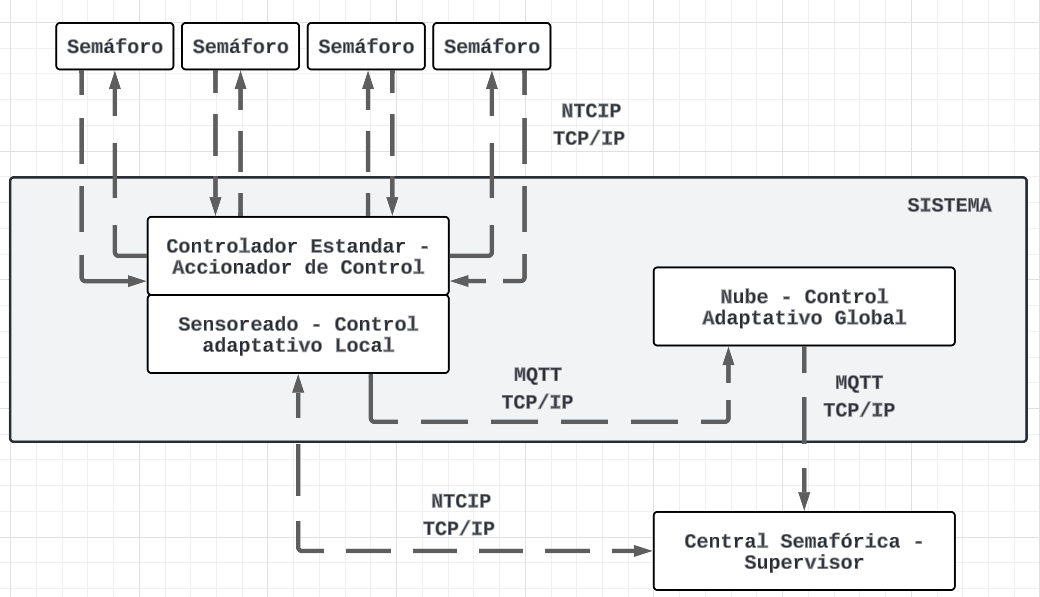
\includegraphics[width=0.9\linewidth,keepaspectratio]{media/image49.png}
  \caption{Diagrama general de flujo del sistema.}
  \label{fig:flujo-general}
  \fuente{Elaboración propia.}
\end{figure}

El módulo IoT actúa como intermediario entre el controlador programable y la nube, facilitando la recolección
y transmisión de datos del entorno local hacia el sistema de control superior. Esta intermediación permite una
comunicación fluida incluso cuando los controladores pertenecen a distintas marcas y protocolos, mitigando la
fragmentación tecnológica existente en Lima, donde coexisten diferentes fabricantes (SICE, SUTEC, ORIUX,
SWARCO) y múltiples protocolos (AENOR, OPCT, NTCIP, BEFA). La Figura~\ref{fig:flujo-completo} detalla la
lógica operativa completa: el sistema inicia con la energización y verificación de la fuente, la inicialización
secuencial del controlador interno, la activación de la cámara, los sensores de monitoreo ambiental y
energético y los actuadores; tras verificar la comunicación, entra en un bucle continuo que captura imágenes,
detecta flujo, velocidad y cola, calcula el índice de congestión, ejecuta la rutina de detección de vehículos
de emergencia y, en su caso, genera la sugerencia de ola verde prioritaria, acondicionando y cifrando los
datos para su transmisión segura a la nube.

\begin{figure}[H]
  \centering
  
\includegraphics[width=0.9\linewidth,keepaspectratio]{media/image66.png}
  
\includegraphics[width=0.9\linewidth,keepaspectratio]{media/image33.png}
  \caption{Diagrama del flujo completo del sistema.}
  \label{fig:flujo-completo}
  \fuente{Elaboración propia.}
\end{figure}

El diagrama de bloques de la solución (Figura~\ref{fig:diagrama-bloques}) evidencia la arquitectura integral
distribuida entre procesamiento local y nube; su leyenda, que separa líneas de alimentación y de señal y
diferencia por colores cada dominio, se presenta en la Figura~\ref{fig:leyenda-bloques}. El sistema se
estructura en torno a la unidad de procesamiento local Raspberry Pi 5, complementada con aceleración o
periféricos de procesamiento de imágenes cuando el desempeño de visión lo requiera, y se conecta con la nube
Azure para análisis, almacenamiento y recomendaciones de coordinación. La alimentación parte de la red de
220\,V AC, protegida por llaves termomagnéticas y disyuntores, convertida mediante una fuente conmutada AC/DC
de 24\,V, complementada con batería DC de respaldo y convertidores DC/DC. El monitoreo ambiental y energético
emplea los sensores INA219 y SHT31, y la captura visual la cámara domo IP con PTZ integrada; la comunicación
opera con NTCIP hacia la central de control y MQTT hacia la nube Azure.

\begin{figure}[H]
  \centering
  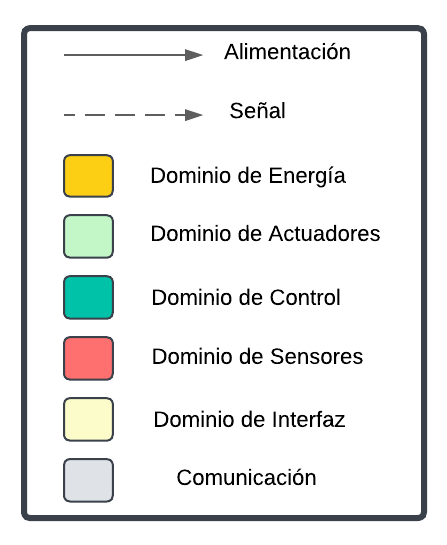
\includegraphics[width=0.9\linewidth,keepaspectratio]{media/image13.png}
  \caption{Leyenda del diagrama de bloques del sistema.}
  \label{fig:leyenda-bloques}
  \fuente{Elaboración propia.}
\end{figure}

\begin{figure}[H]
  \centering
  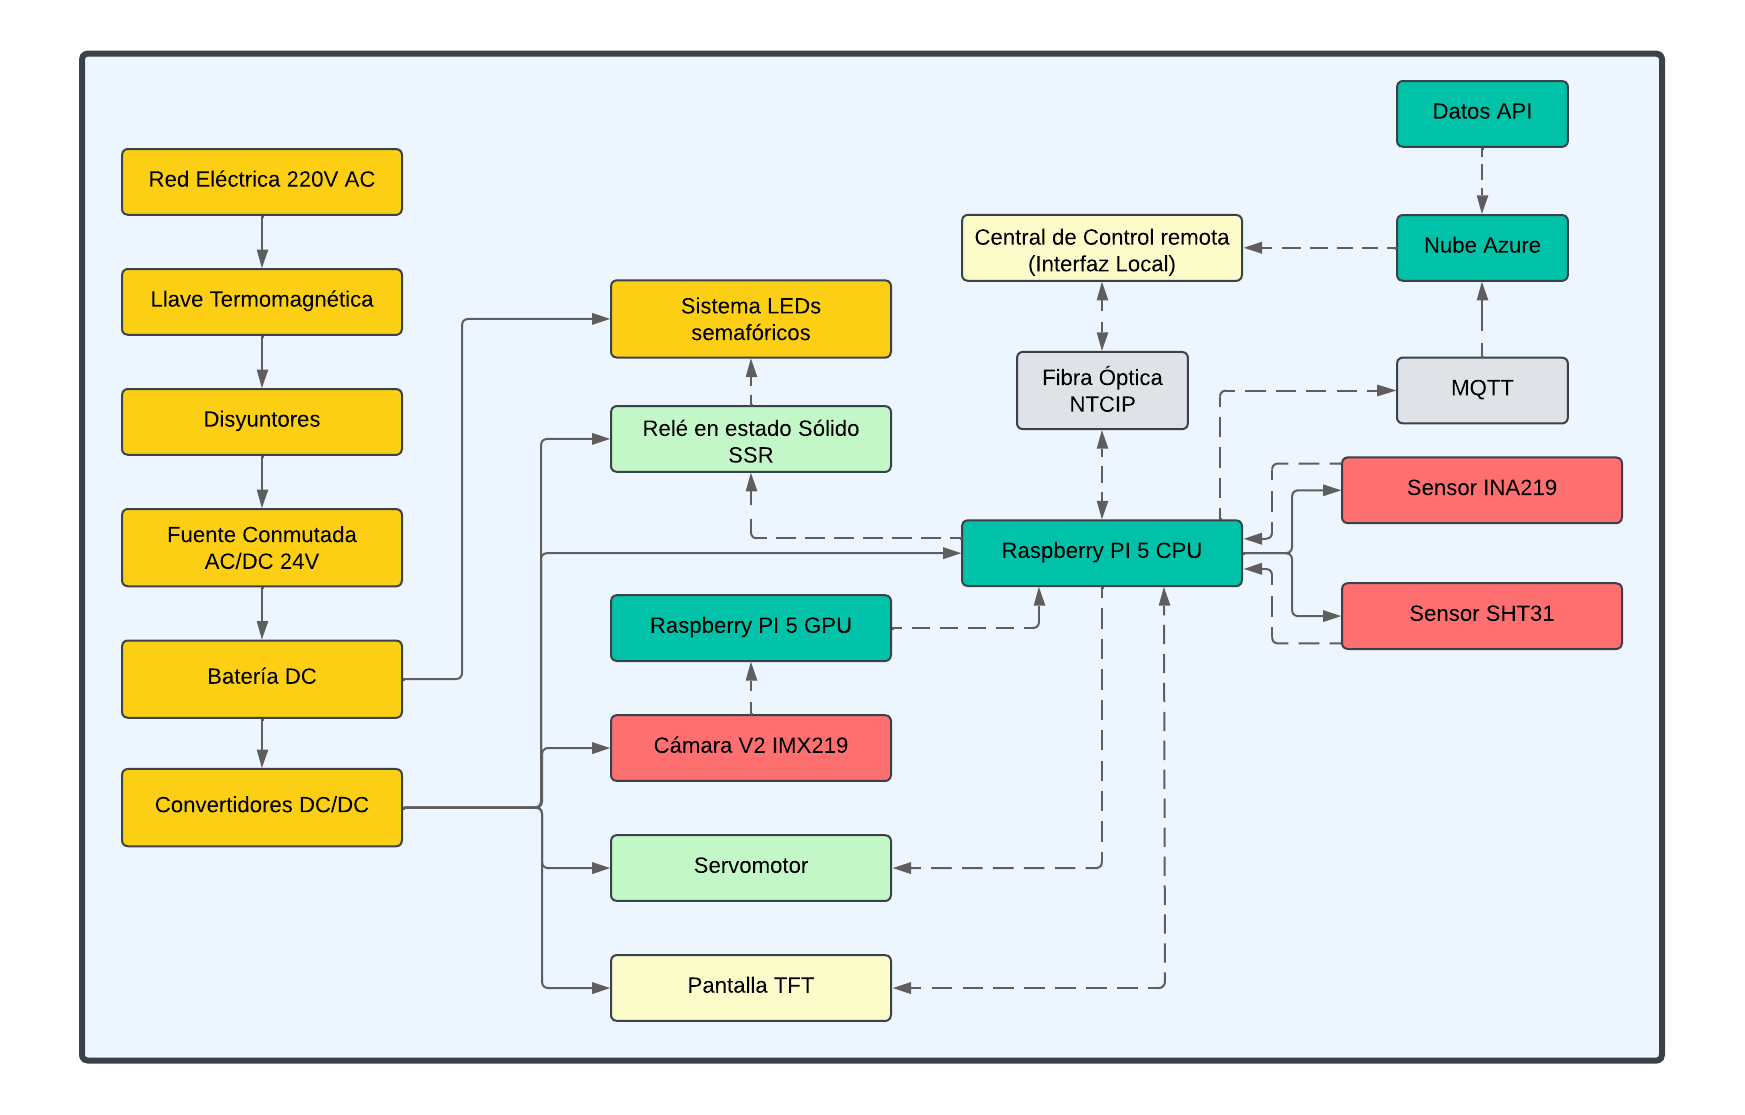
\includegraphics[width=0.9\linewidth,keepaspectratio]{media/image151.png}
  \caption{Diagrama de bloques del sistema.}
  \label{fig:diagrama-bloques}
  \fuente{Elaboración propia.}
\end{figure}

\subsection{Jerarquía de alcance y responsabilidad}\label{sec:jerarquia-alcance}

La solución se organiza en niveles de alcance que separan el núcleo validado de los módulos exploratorios. La
relación \emph{edge}--nube--controlador es jerárquica: la cámara y los sensores alimentan la estimación y el
control difuso en el borde; el borde envía telemetría segura a la nube (supervisión, históricos y coordinación)
y recomendaciones acotadas al controlador semafórico, que conserva la autoridad final sobre luces y
enclavamientos; la nube y la central devuelven únicamente parámetros autorizados. La
Tabla~\ref{tab:niveles-alcance} detalla los niveles y la evidencia esperada de cada uno.

\begin{table}[H]
  \centering
  \caption{Niveles de alcance del sistema y evidencia esperada.}
  \label{tab:niveles-alcance}
  \begin{tabularx}{\linewidth}{@{}>{\raggedright\arraybackslash}p{3.5cm}>{\raggedright\arraybackslash}X>{\raggedright\arraybackslash}p{4.6cm}@{}}
    \toprule
    \textbf{Nivel} & \textbf{Contenido} & \textbf{Evidencia esperada}\\
    \midrule
    Nivel 1: núcleo validado & Sensado/variables equivalentes, ICV, control difuso local, diseño electrónico y mecánico, SUMO y comparación con línea base. & Ecuaciones, reglas, esquemas, CAD, simulaciones y tabla comparativa.\\
    Nivel 2: arquitectura de soporte & Comunicación con nube, supervisión, histórico, alertas y actualización autorizada de parámetros. & Arquitectura, mensajes, dashboard y prueba controlada.\\
    Nivel 3: seguridad y operación & Modelo de amenazas, cifrado, autenticación, roles, logs, validación de parámetros y modos degradados. & Tabla de amenazas, flujo de confianza y casos negativos.\\
    Nivel 4: módulos exploratorios/futuros & Aprendizaje por refuerzo, CNN--LSTM, optimización metropolitana, reentrenamiento continuo e integración comercial certificada. & Propuesta o experimento separado; no condiciona el objetivo general.\\
    \bottomrule
  \end{tabularx}
  \fuente{Elaboración propia.}
\end{table}

\subsection{Riesgos y limitaciones del concepto edge--nube}\label{sec:riesgos-concepto}

La arquitectura seleccionada presenta riesgos y limitaciones que condicionan su implementación y se gestionan
con las mitigaciones de la Tabla~\ref{tab:riesgos-concepto}. Estas mitigaciones se trazan con los
requerimientos verificables (Tabla~\ref{tab:req-verificables}) y se ejercitan durante la validación.

\begin{table}[H]
  \centering
  \caption{Riesgos y limitaciones del concepto edge--nube y sus mitigaciones.}
  \label{tab:riesgos-concepto}
  \begin{tabularx}{\linewidth}{@{}>{\raggedright\arraybackslash}p{3.6cm}>{\raggedright\arraybackslash}X>{\raggedright\arraybackslash}p{2.0cm}@{}}
    \toprule
    \textbf{Riesgo o limitación} & \textbf{Mitigación de diseño} & \textbf{Requisito}\\
    \midrule
    Pérdida de conectividad con la nube & Decisión local en el borde y retorno determinista al plan base; almacenamiento local y reintento de conexión. & R-C01, R-C04, R-VAL03\\
    Falla o descalibración de sensores/cámara & Diagnóstico interno, modo degradado ante datos inválidos y pruebas periódicas de calibración. & R-C04, R-F01\\
    Oclusión o geometría irregular de la intersección & Calibración geométrica, ajuste de zonas de detección y verificación de cobertura en campo. & R-MEC03\\
    Errores del algoritmo de optimización & Recomendaciones acotadas por límites de fase; el controlador valida antes de aplicar y mantiene la autoridad final. & R-C02, R-C03\\
    Ciberataque o manipulación de parámetros & Cifrado en tránsito, identidad por dispositivo, lista blanca de parámetros, roles y registro de eventos. & R-SEC01--R-SEC04, R-COM02\\
    Transitorios eléctricos y cortes de energía & Protecciones dimensionadas y respaldo por batería/UPS para apagado controlado. & R-ELEC01, R-ELEC02\\
    Heterogeneidad de controladores en Lima & Módulo IoT como intermediario que abstrae marcas y protocolos sin sustituir la lógica local. & R-COM01, R-OP01\\
    Sobrecosto frente al presupuesto objetivo & Componentes disponibles y de bajo costo; estimación de CAPEX/OPEX y análisis de sensibilidad. & R-COST01\\
    \bottomrule
  \end{tabularx}
  \fuente{Elaboración propia.}
\end{table}

\section{Matriz de trazabilidad de objetivos}\label{sec:trazabilidad-objetivos}

Finalmente, la Tabla~\ref{tab:trazabilidad} vincula los objetivos específicos con los requerimientos, los
capítulos donde se abordan, el método de validación y la evidencia esperada, cerrando la trazabilidad entre el
diseño conceptual y las etapas de desarrollo y validación.

\begin{landscape}
\footnotesize
\begin{longtable}{@{}p{1.3cm}p{4.3cm}p{2.6cm}p{3.7cm}p{7.0cm}@{}}
\caption{Trazabilidad entre objetivos, requerimientos y evidencia.}\label{tab:trazabilidad}\\
\toprule
\textbf{Objetivo} & \textbf{Requerimientos relacionados} & \textbf{Capítulos} & \textbf{Método de validación} & \textbf{Evidencia/resultado}\\
\midrule
\endfirsthead
\toprule
\textbf{Objetivo} & \textbf{Requerimientos relacionados} & \textbf{Capítulos} & \textbf{Método de validación} & \textbf{Evidencia/resultado}\\
\midrule
\endhead
\bottomrule
\endfoot
OE1 & Base para todos los requerimientos & 1 y 2 & Revisión comparativa y síntesis & Tabla de lecciones y criterios adoptados.\\
OE2 & R-F01 a R-COST01 & 3 & Inspección de especificación & Tabla~\ref{tab:req-verificables} con código, criterio, justificación y verificación.\\
OE3 & R-C01, R-C02, R-C04, R-COM01, R-MEC01 & 3 & Evaluación ponderada & Caja negra, estructura funcional, matriz morfológica y concepto C.\\
OE4 & R-ELEC01 a R-ELEC03, R-COM01 & 4 & Cálculo y revisión de diseño & Esquemas, consumo, selección de componentes y protecciones.\\
OE5 & R-MEC01 a R-MEC03 & 5 & CAD, cálculo y simulación & Distribución, soporte, análisis térmico/estructural y factor de seguridad.\\
OE6 & R-F02, R-C01, R-C03, R-C04 & 6 & Casos de prueba y SUMO & Membresías, reglas, superficie, saturaciones y modos degradados.\\
OE7 & R-COM01, R-COM02, R-NUB01 & 6 y 7 & Demostración controlada & Flujo de mensajes, histórico, alertas y prueba de desconexión.\\
OE8 & R-SEC01 a R-SEC04 & 2, 6 y 7 & Análisis de amenazas & Tabla de amenazas, mitigaciones y evidencia de controles propuestos.\\
OE9 & R-VAL01 a R-VAL03 & 7 & Simulación comparativa & Tabla comparativa de métricas SUMO y archivos de salida del Capítulo~7.\\
OE10 & R-COST01 & 7 & Presupuesto y sensibilidad & CAPEX/OPEX con fuentes, fecha y supuestos.\\
\bottomrule
\end{longtable}
\fuente{Elaboración propia.}
\end{landscape}
